\documentclass[fleqn]{jbook}
\usepackage{physpub}

\begin{document}

\begin{question}{専攻 問題5}{}

物質の結晶構造や格子定数を求めたり、単結晶の方位を調べる簡便な方法として用いられるX線回折写真法の代表的なものに、ラウエ法とデバイ・シュラー法がある。これらは、その目的、用いるX線の種類、試料などに顕著な違いがある。

\begin{subquestions}
\SubQuestion
上記の2方法のそれぞれについて、その目的、用いるX線、試料の別を述べよ。
\end{subquestions}

結晶の単位胞(単位格子)の3稜を表す基本ベクトル$\Vec{a_1}$,$\Vec{a_2}$,$\Vec{a_3}$と
\[ \Vec{a_i}\cdot \Vec{b_j}=\delta_{ij}\]
の関係にあるベクトル$\Vec{b_1}$,$\Vec{b_2}$,$\Vec{b_3}$を基本ベクトルとする格子を逆格子という。また、$g_1$,$g_2$,$g_3$を整数とするとき、ベクトル
\[ \Vec{g}=g_1\Vec{b_1}+g_2\Vec{b_2}+g_3\Vec{b_3} \]
を逆格子ベクトルという。結晶の格子面(原子面)を表すのには、ミラー指数が用いられる。ミラー指数$(g_1,g_2,g_3)$で表される格子面は、逆格子ベクトル$\Vec{g}$に垂直であり、互いに素なミラー指数$(g_1,g_2,g_3)$で表される格子面の面間隔は、
\[ d=1/|\Vec{g}| \]
で与えられる。

入射X線および、反射X線の波数ベクトルをそれぞれ、$\Vec{k_0}$および$\Vec{k}$とすると、結晶による強い回折が起きる条件はラウエの条件
\[ \Vec{k}-\Vec{k_0}=\Vec{g} \]
で与えられる。ここで、$\Vec{g}$は任意の逆格子ベクトルである。

\begin{subquestions}[2]
\SubQuestion
ラウエの条件からブラッグの条件が導かれることを示せ。
\end{subquestions}

単位胞の中に$n$個の原子を含む結晶からの回折線の振幅は、原子$i$の原子散乱因子を$f_i(\Vec{g})$として、構造因子
\[ F(\Vec{g})=\sum_{i=1}^n f(\Vec{g})\exp(2\pi i \Vec{g}\cdot \Vec{r_i}) \]
に比例する。ここで、$\Vec{r_i}$は、原子$i$の位置ベクトルである。

\begin{subquestions}[3]
\SubQuestion
\parbox[t]{70mm}{
右図のように単位胞をとるとき、面心立方(fcc)構造および体心立方(bcc)構造のそれぞれについて、波長$\lambda$のX線ブラッグ反射のミラー指数をブラッグ角の小さい方から3つずつ挙げよ。ただし、結晶学的に同等な反射はひとつと数える。}\parbox[t]{50mm}{\vspace*{-5mm}
\begin{center}
\includegraphics[clip,height=45mm,width=40mm]{1997phy5-1.eps}
\end{center}
}\parbox[t]{50mm}{\vspace*{-5mm}
\begin{center}
\includegraphics[clip,height=45mm,width=40mm]{1997phy5-2.eps}
\end{center}
}
\end{subquestions}

\parbox[t]{110mm}{右の表は、銅(fcc構造)および鉄(bcc構造)を試料として、回折されたモリブデンの${\rm{K}}_\alpha$線(波長0.71Å)について、$\sin\theta_B$($\theta_B$はブラッグ角)の値を小さい方から4つ並べたものである。}\parbox[t]{50mm}{\vspace*{-7mm}
\begin{center}
\begin{tabular}{|c|c|c|}\hline
順位 & 試料A & 試料B \\ \hline 
1 & 0.175 & 0.170 \\ \hline
2 & 0.248 & 0.196 \\ \hline 
3 & 0.303 & 0.278 \\  \hline
4 & 0.350 & 0.326 \\ \hline
\end{tabular}
\end{center}
}

\begin{subquestions}[4]
\SubQuestion
試料Aは銅・鉄のどちらか。
\end{subquestions}

\parbox[t]{110mm}{
NaClは岩塩型(右図)の結晶構造をなし、正イオンあるいは負イオンのみがつくる副格子はともに面心立方格子である。下図は、NaClによって回折された銅の${\rm{K}}_\alpha$線の強度分布である。}\parbox[t]{50mm}{\vspace*{-10mm}
\begin{center}
\includegraphics[clip,height=40mm,width=40mm]{1997phy5-3.eps}
\end{center}
}

\begin{subquestions}[5]
\SubQuestion
下図において、ピーク1・4の強度は、2・3・5に比べて極端に小さい。このような強度分布が現れる理由を説明せよ。

\begin{center}
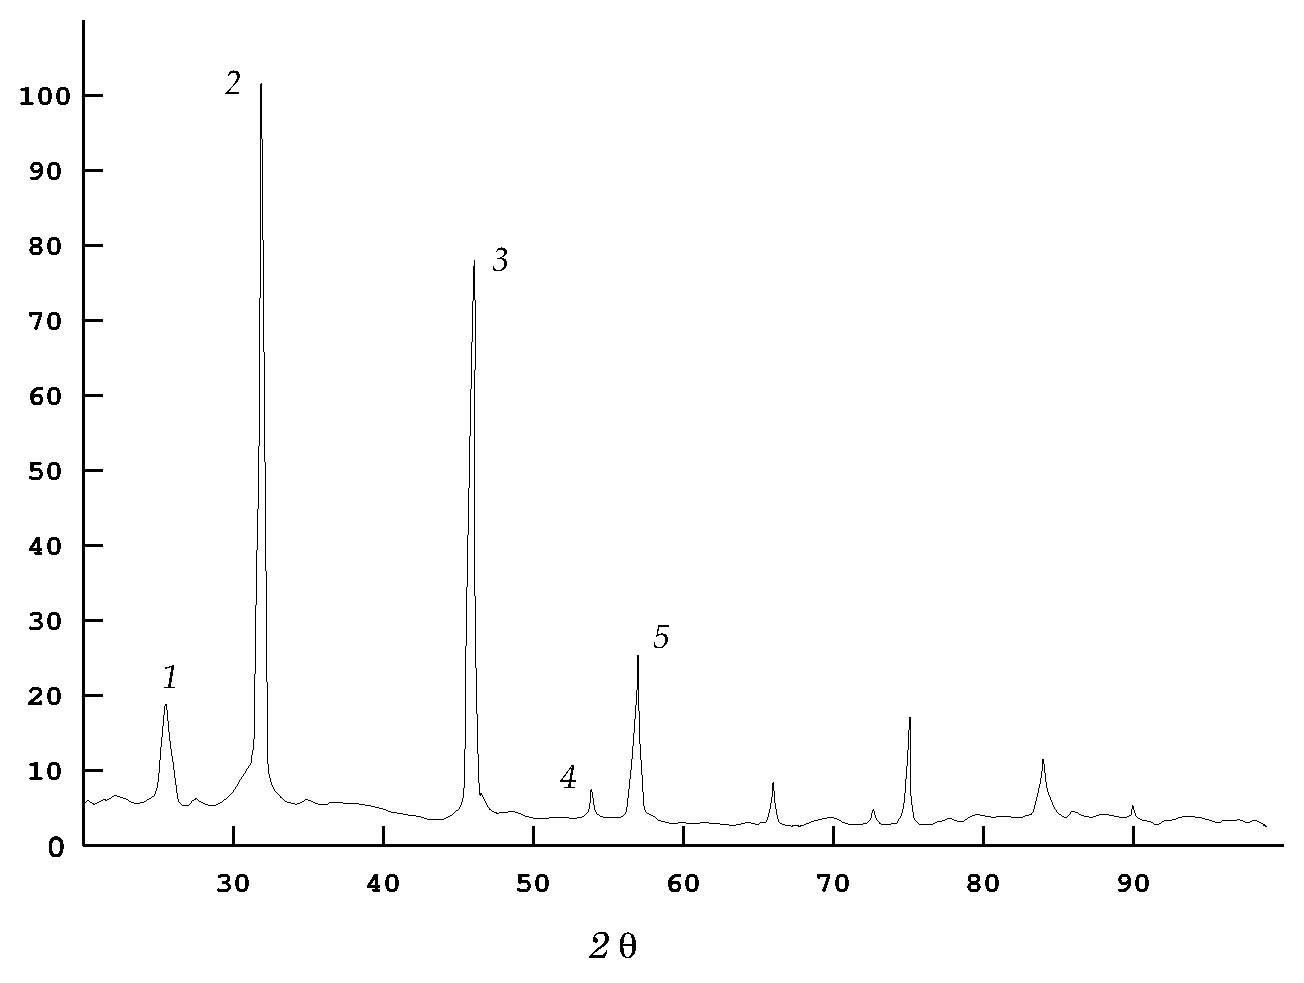
\includegraphics[clip,height=70mm,width=100mm]{1997phy5-4.eps}
\end{center}

\end{subquestions}
\end{question}
\begin{answer}{専攻 問題5}{}
\begin{subanswers}

\SubAnswer  
まとめると次のようになる。
 
\begin{tabular}{|c||p{5cm}|p{5cm}|} \hline
    & ラウエ法 & デバイ・シュラー法 \\ \hline\hline
目的& 結晶の対称性を調べたり、既知結晶の方向を調べる。& 結晶の格子定数・構造等を決定する。\\ \hline
用いるX線  & 連続X線(白色X線) & 単色X線 \\ \hline
試料 & 単結晶 & 粉末状結晶  \\ \hline
\end{tabular}

\SubAnswer
\parbox[t]{100mm}{
$\Vec{g}=(ng_1,ng_2,ng_3)=n\Vec{g_0}$の形に、$g_1,g_2,g_3$が互いに素になるような整数$n$をとる。$|\Vec{k}|=|\Vec{k_0}|=\frac{1}{\lambda}$なので、
\[ |\Vec{k}-\Vec{k_0}|^2=|\Vec{g}|^2 \Longleftrightarrow 4\frac{1}{\lambda}^2 \sin^2\theta =\frac{n^2}{d^2} \Longleftrightarrow n\lambda =2d\sin\theta \]
よって、ブラッグの反射の公式が得られた。}\parbox[t]{60mm}{\vspace*{-10mm}
\begin{center}
\includegraphics[clip,height=30mm,width=50mm]{1997phy5-5.eps}
\end{center}
}

\SubAnswer
今、bcc(体心立方)の単位胞として図の立方体を考える。 この単位胞には2つの同種粒子が$(0,0,0)$と$(\frac{1}{2},\frac{1}{2},\frac{1}{2})$に入っていると考えられるので、$f_{(0,0,0)}(\Vec{g})=f_{(\frac{1}{2},\frac{1}{2},\frac{1}{2})}(\Vec{g}) \equiv f(g)$として、
\begin{eqnarray*} 
F(\Vec{g})& = & f(g)\{1+\exp(i\pi(g_1+g_2+g_3)) \\
    & = & f(g)\times
\left\{ \begin{array}{ccl}
0 & \quad & g_1+g_2+g_3={\mbox{Odd}} \\
2 & \quad & g_1+g_2+g_3={\mbox{Even}} 
\end{array}\right.
\end{eqnarray*}

$|\Vec{g_1}|<|\Vec{g_2}| \Longleftrightarrow |\theta_1|<|\theta_2|$から、$|\Vec{g}|$の小さいものから3つ挙げれば良い。但し、$g_1,g_2,g_3$の入れ替えの組み合わせで等しくなったり、正負が逆転しているものは、同等な反射となるので、除かなければならない。また、$F(\Vec{g})$が$0$になり上の消滅則を満たすものは、反射しないことを意味するので除かねばならない。よって、求めるミラー指数は$(1,1,0),(2,0,0),(2,1,1)$である。

fccの場合も、同様に3つの同種粒子が存在していると考えて、
\begin{eqnarray*}
F(\Vec{g}) & = & f(g)(1+\exp(i\pi(g_2+g_3))+\exp(i\pi(g_3+g_1))+\exp(i\pi(g_1+g_2)) \\
           & = & f(g)(1+(-1)^{(g_2+g_3)}+(-1)^{(g_3+g_1)}+(-1)^{(g_1+g_2)}) \\
           & = & f(g)\times\left\{
\begin{array}{cclcl} 
4 & \quad & g_1,g_2,g_3 & \quad & {\mbox{All Odd}} \quad or \quad   {\mbox{All Even}} \\
0 & \quad & g_1,g_2,g_3 & \quad & {\mbox{Otherwise}} \\
\end{array}\right.
\end{eqnarray*}
bccと同様にして、求めるミラー指数は、$(1,1,1),(2,0,0),(2,2,0)$となる。

\SubAnswer
\parbox[t]{70mm}{{\bf{2}}の計算から、{\bf{3}}でもとめたブラッグ角$\theta_B$の小さいものから、$\theta_{B1},\theta_{B2}$とすると、$\sin\theta_B$の比は、
\[ \frac{\sin\theta_{B1}}{\sin\theta_{B2}}=\frac{|\Vec{g_1}|}{|\Vec{g_2}|} \]
の関係があるので、与えられた表の数値について、計算すると、右表のようになる。}
\parbox[t]{80mm}{\vspace*{-5mm}
\begin{center}
\begin{tabular}{|c||c|c|c|c|} \hline
  & $\frac{\sin\theta_{B1}}{\sin\theta_{B2}}$ &  $\frac{\sin\theta_{B3}}{\sin\theta_{B1}}$ & $2\frac{\sin\theta_{B1}}{\sin\theta_{B2}}$ & $\frac{\sin\theta_{B3}}{\sin\theta_{B1}}$ \\ \hline\hline
A & 1.417 & 1.731 & 1.411 & 1.221 \\ \hline
B & 1.152 & 1.635 & 1.734 & 1.418 \\ \hline\hline
bcc & $\sqrt{2}$ & $\sqrt{3}$ & &  \\ \hline
fcc &      &    & $\sqrt{3}$ & $\sqrt{2}$ \\ \hline
\end{tabular}\end{center}
}

よって、Aをbcc、Bをfccと判断すべきである。よって、Aが鉄である。
\SubAnswer
{\bf{3}}と同様にして、図の立方体を単位胞と考えると、$\forall f_i(\Vec{g})\{\Vec{r_i}に{\rm{Cl}}原子が存在している。\} \equiv f_{\rm{Cl}}$、$\forall f_i(\Vec{g})\{\Vec{r_i}に{\rm{Na}}原子が存在している。\} \equiv f_{\rm{Na}}$と書くことにすると、
\begin{eqnarray*}
F(\Vec{g}) & = & f_{\rm{Cl}}(1+(-1)^{g_2+g_3}+(-1)^{g_3+g_1}+(-1)^{g_1+g_2})+f_{\rm{Na}}((-1)^{g_1}+(-1)^{g_2}+(-1)^{g_3}+(-1)^{g_1+g_2+g_3}) \\
    & = & \left\{ \begin{array}{ccc}
4(f_{\rm{Na}}+f_{\rm{Cl}}) & \quad & {\mbox{All Even}} \\
4(f_{\rm{Na}}-f_{\rm{Cl}}) & \quad & {\mbox{All Odd}} \\
0                          & \quad & {\mbox{Otherwise}} 
\end{array}\right.
\end{eqnarray*}
\parbox[t]{70mm}{
\rm{Na}、\rm{Cl}に対して散乱因子が大きく異なる原因は考えられないから、$|f_{\rm{Na}}+f_{\rm{Cl}}|>|f_{\rm{Na}}-f_{\rm{Cl}}|$と考えるのが正しいと思われる。すると$|\Vec{g}|$の小さいものから順に、
右表の通り、偶奇性とピークの大小の対応がとれており、上の推定が正しく、強度分布を説明できたことになる。}\parbox[t]{100mm}{\vspace*{-10mm}
\begin{center}
\begin{tabular}{|p{20mm}|p{20mm}|p{30mm}|} \hline
$\Vec{g}$ & $F(\Vec{g})$の条件 & 読み取りのピークの大きさ \\ \hline\hline
$(1,1,1)$ & {\mbox{All odd}}  &  小  \\ \hline
$(2,0,0)$ & {\mbox{All Even}} &  大  \\ \hline
$(2,2,0)$ & {\mbox{All Even}} &  大  \\ \hline
$(3,1,1)$ & {\mbox{All Odd}}  &  小  \\ \hline
$(2,2,2)$ & {\mbox{All Even}}  &  大  \\ \hline
\end{tabular}\end{center}}
 
\end{subanswers}
\end{answer}

\end{document}
